\subsection{Run on The Cancer Genomics Atlas}
The same pipeline described so far can be applied at other datasets. In this section, the hSBM model is run on some samples from the TCGA. The principle is the same, but here samples come from cancer tissues, so there must be more complexity and variability behind the data. Moreover, being able to separate cancer samples is not always easy clinically and develop a method to do this can be fascinating and useful for the scientific community~\cite{Farver2018}. 

First of all, let's take a look at the V-measure scores. As shown in figure~\ref{fig:topic/tcga/metric} the maximum score is $\simeq 0.8$, which is quite good, comparable with the healthy GTEx scenario. The publishers of the dataset~\cite{Farver2018} obtained similar score considering just homogeneity. In this dataset, there isn't a sub-tissue label as before, but a \textit{disease type} cancer information is available. The disease type separation happens but obtain a lower score; the fact that there is no evident difference between Zipf's laws when separating data by disease type (previously shown in figure~\ref{fig:structure/tcga/fraction_of_trascriptome_disease}) means that all genes contribute to define this specific label. The hierarchic approach which separates firstly tissues and then cancer type is here necessary and useful. In fact, looking at the label \textit{disease tissue} that considers the cancer types inside each tissue the result is very encouraging. In fact the score is quite high and the results promising. To gain better scores in this situation where samples are affected by the cancer complexity and heterogeneity is probably necessary to add more genes to the network. 
\begin{figure}[htb!]
    \centering
    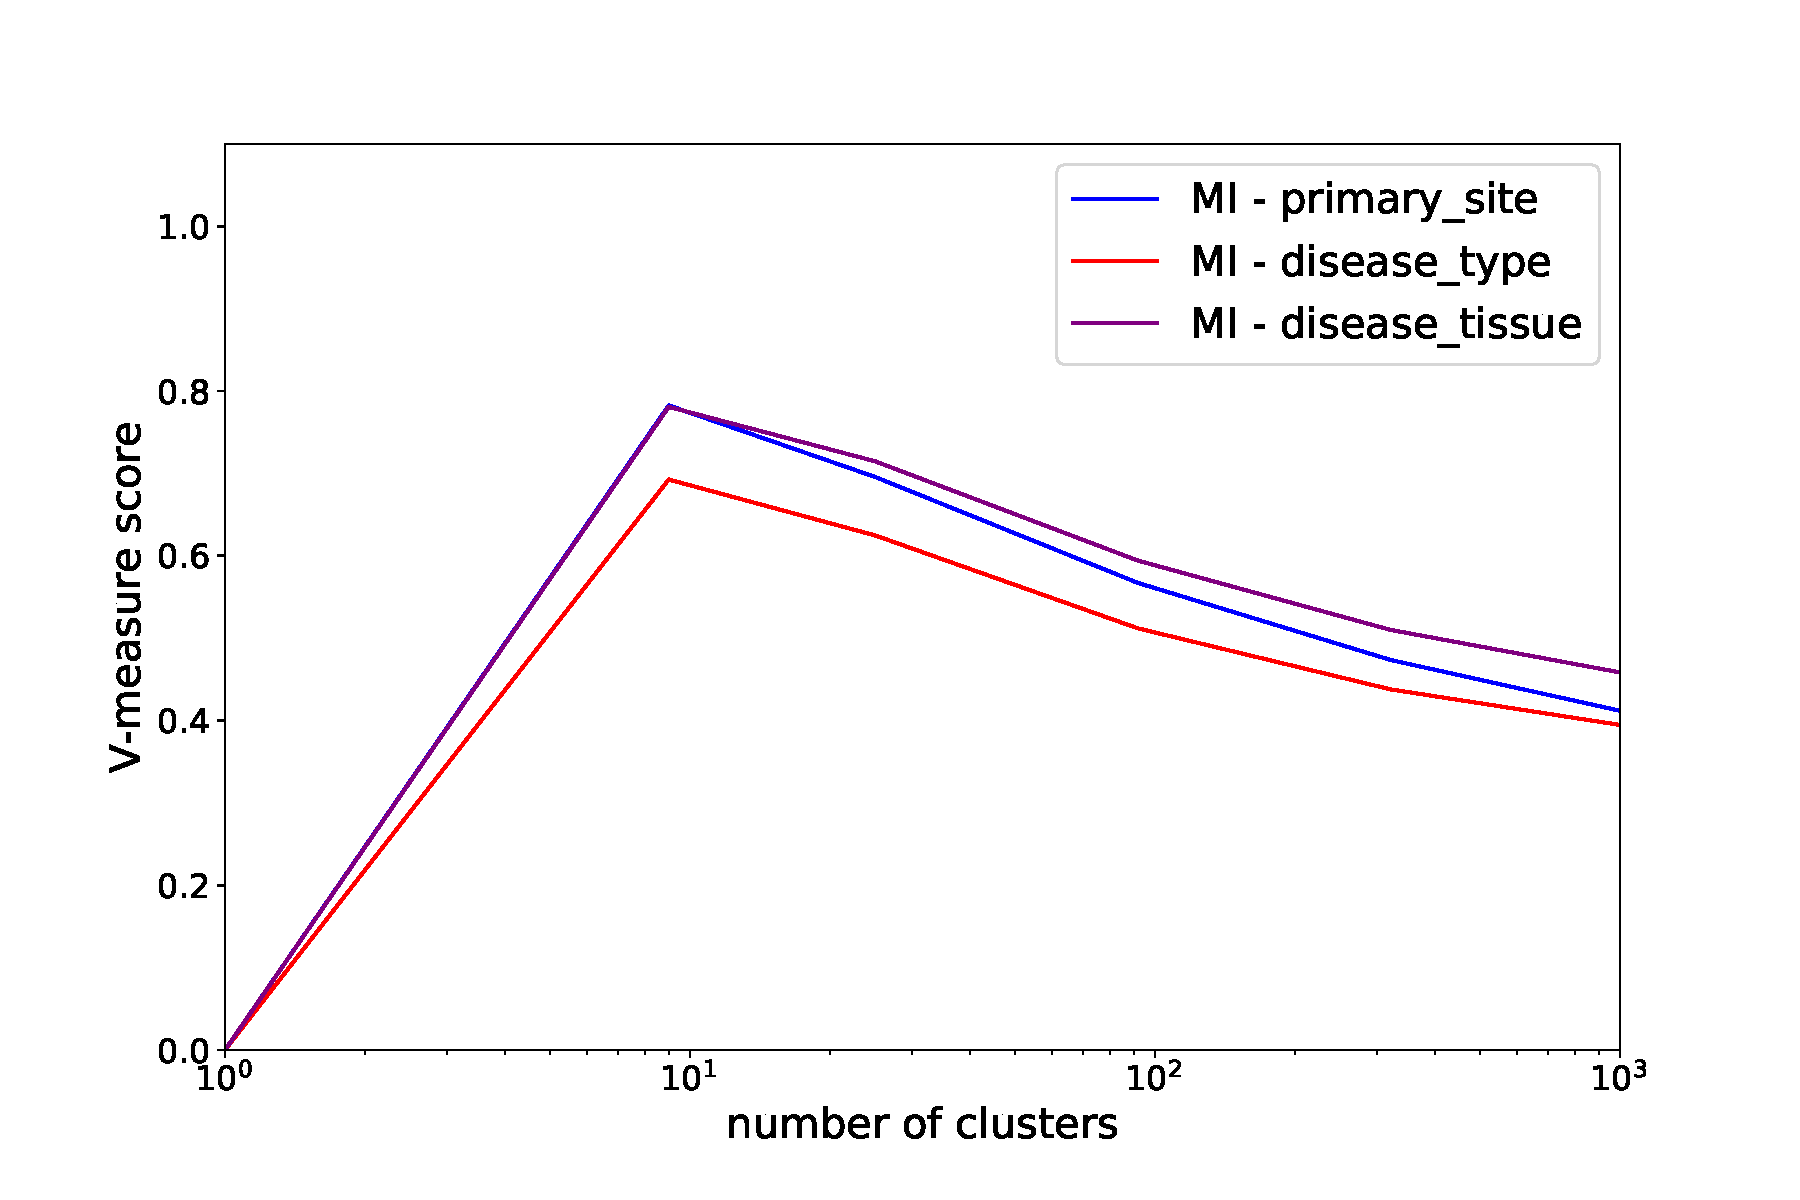
\includegraphics[width=0.85\linewidth]{pictures/topic/tcga/metric.pdf}
    \caption{Score across the hierarchy for TCGA. In blue the primary site labels were considered, in red the disease types and in purple the mix of the two.}
    \label{fig:topic/tcga/metric}
\end{figure}
\FloatBarrier
Looking directly into the cluster composition the tissue separation is quite good and visually appreciable. In figure~\ref{fig:topic/tcga/fraction_clustercomposition_l4_primary_site} clusters at the higher level of the hierarchy. Some tissues are well separated at this point, at the same time the model seems to group the samples by system: digestive system is the more evident.
\begin{figure}[htb!]
	\centering
	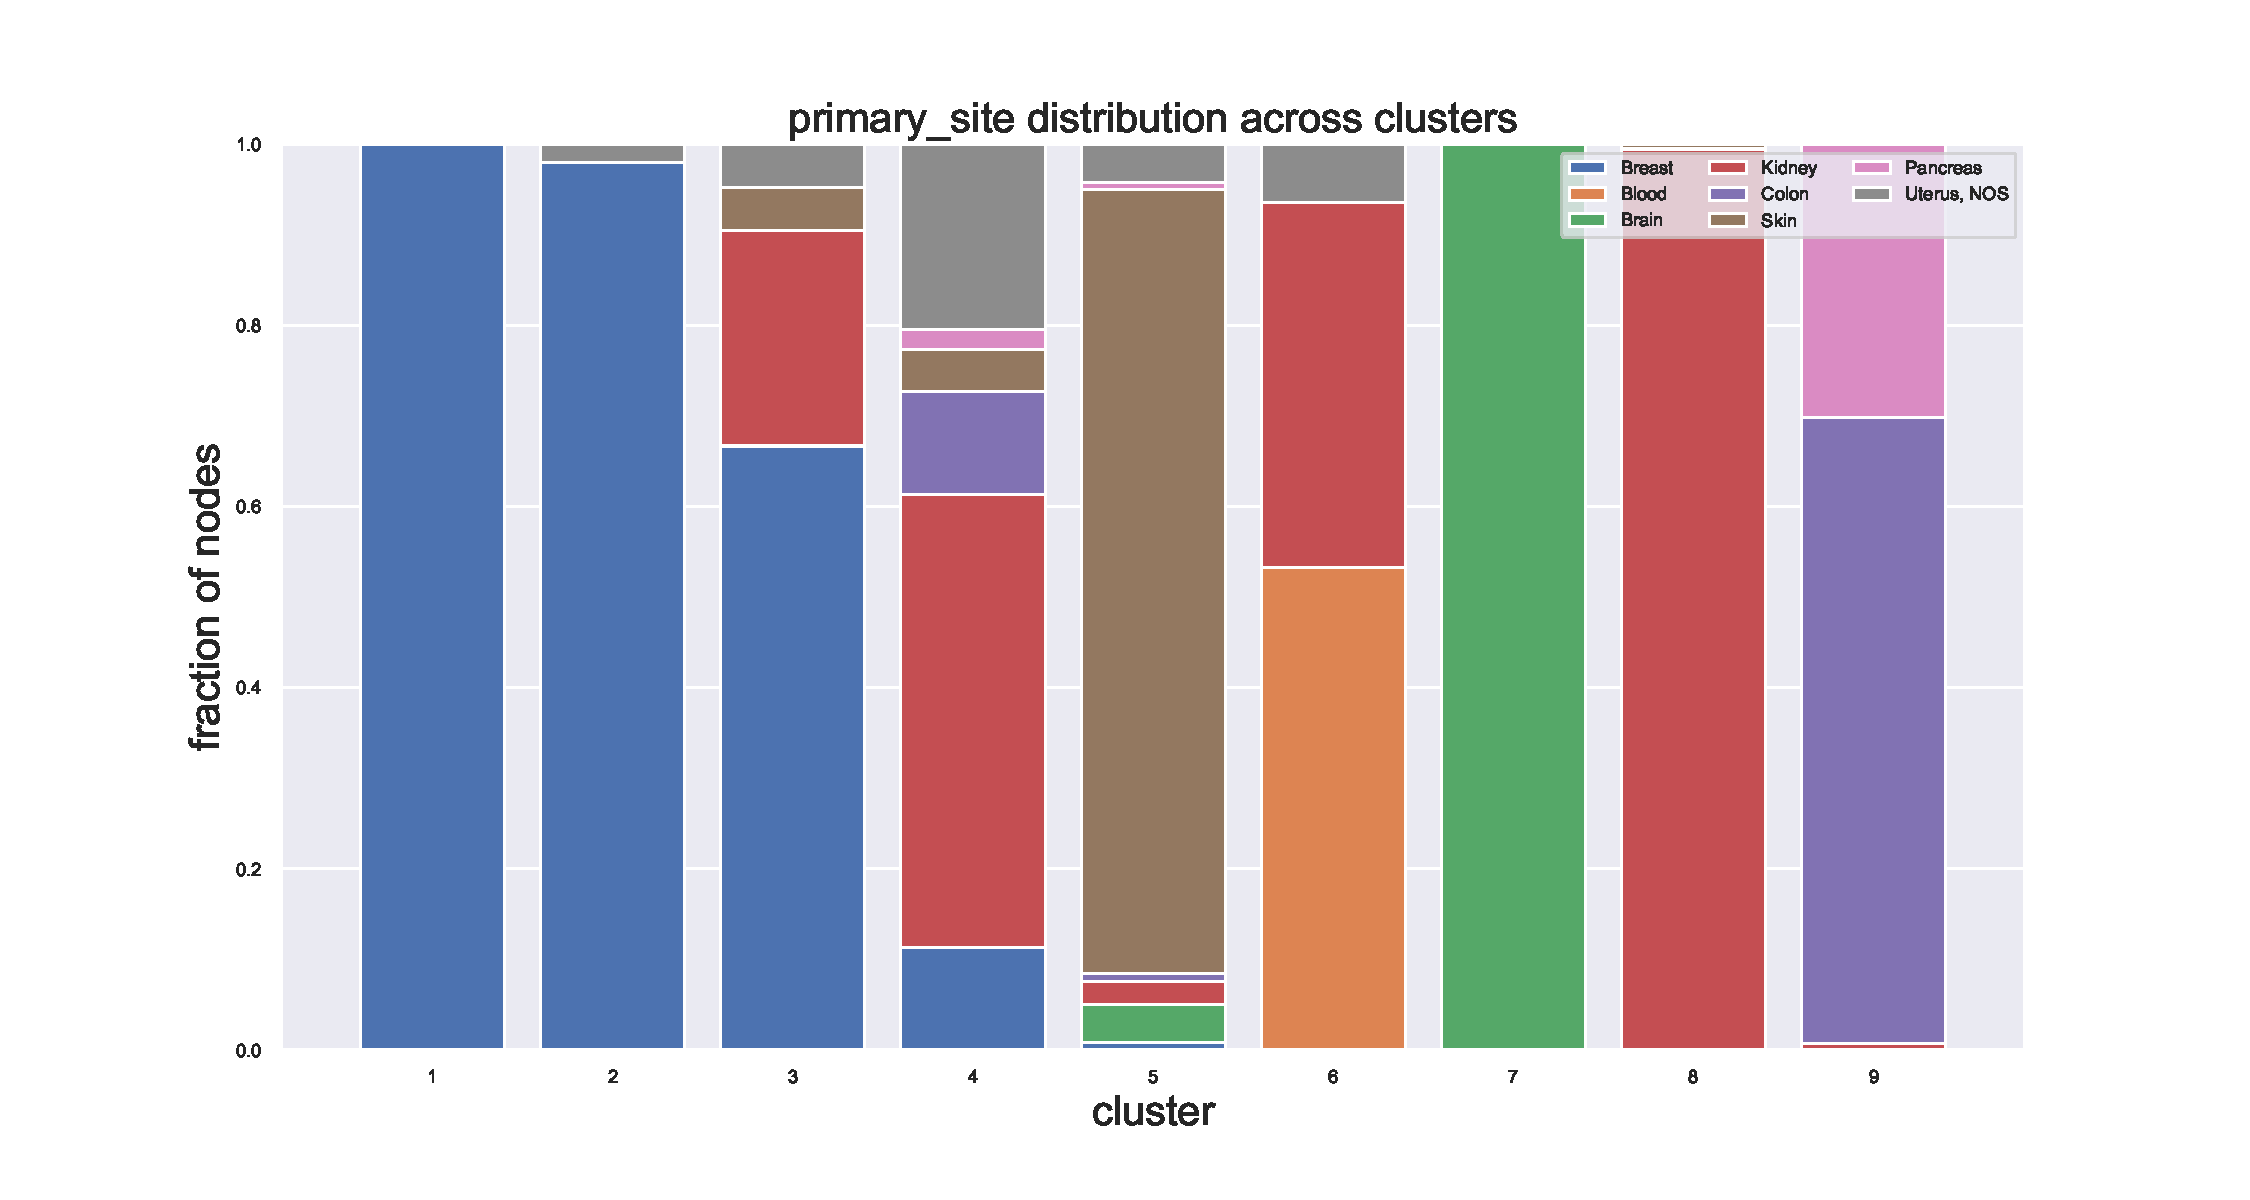
\includegraphics[width=0.9\linewidth]{pictures/topic/tcga/fraction_clustercomposition_l4_primary_site.pdf}
	\caption{Clusters of diseased tissues at the higher level of the hierarchy. Breast is well separated, such as skin and brain. Cluster 9 contains digestive systems samples from pancreas and colon.}
	\label{fig:topic/tcga/fraction_clustercomposition_l4_primary_site}
\end{figure}
Going deeper in the hierarchy the tissue separation becomes visually appreciable and all the clusters are almost tissue-specific. This is clear in figure~\ref{fig:topic/tcga/fraction_clustercomposition_l3_primary_site} which shows the primary site of the tumours well classified.
\begin{figure}[htb!]
	\centering
	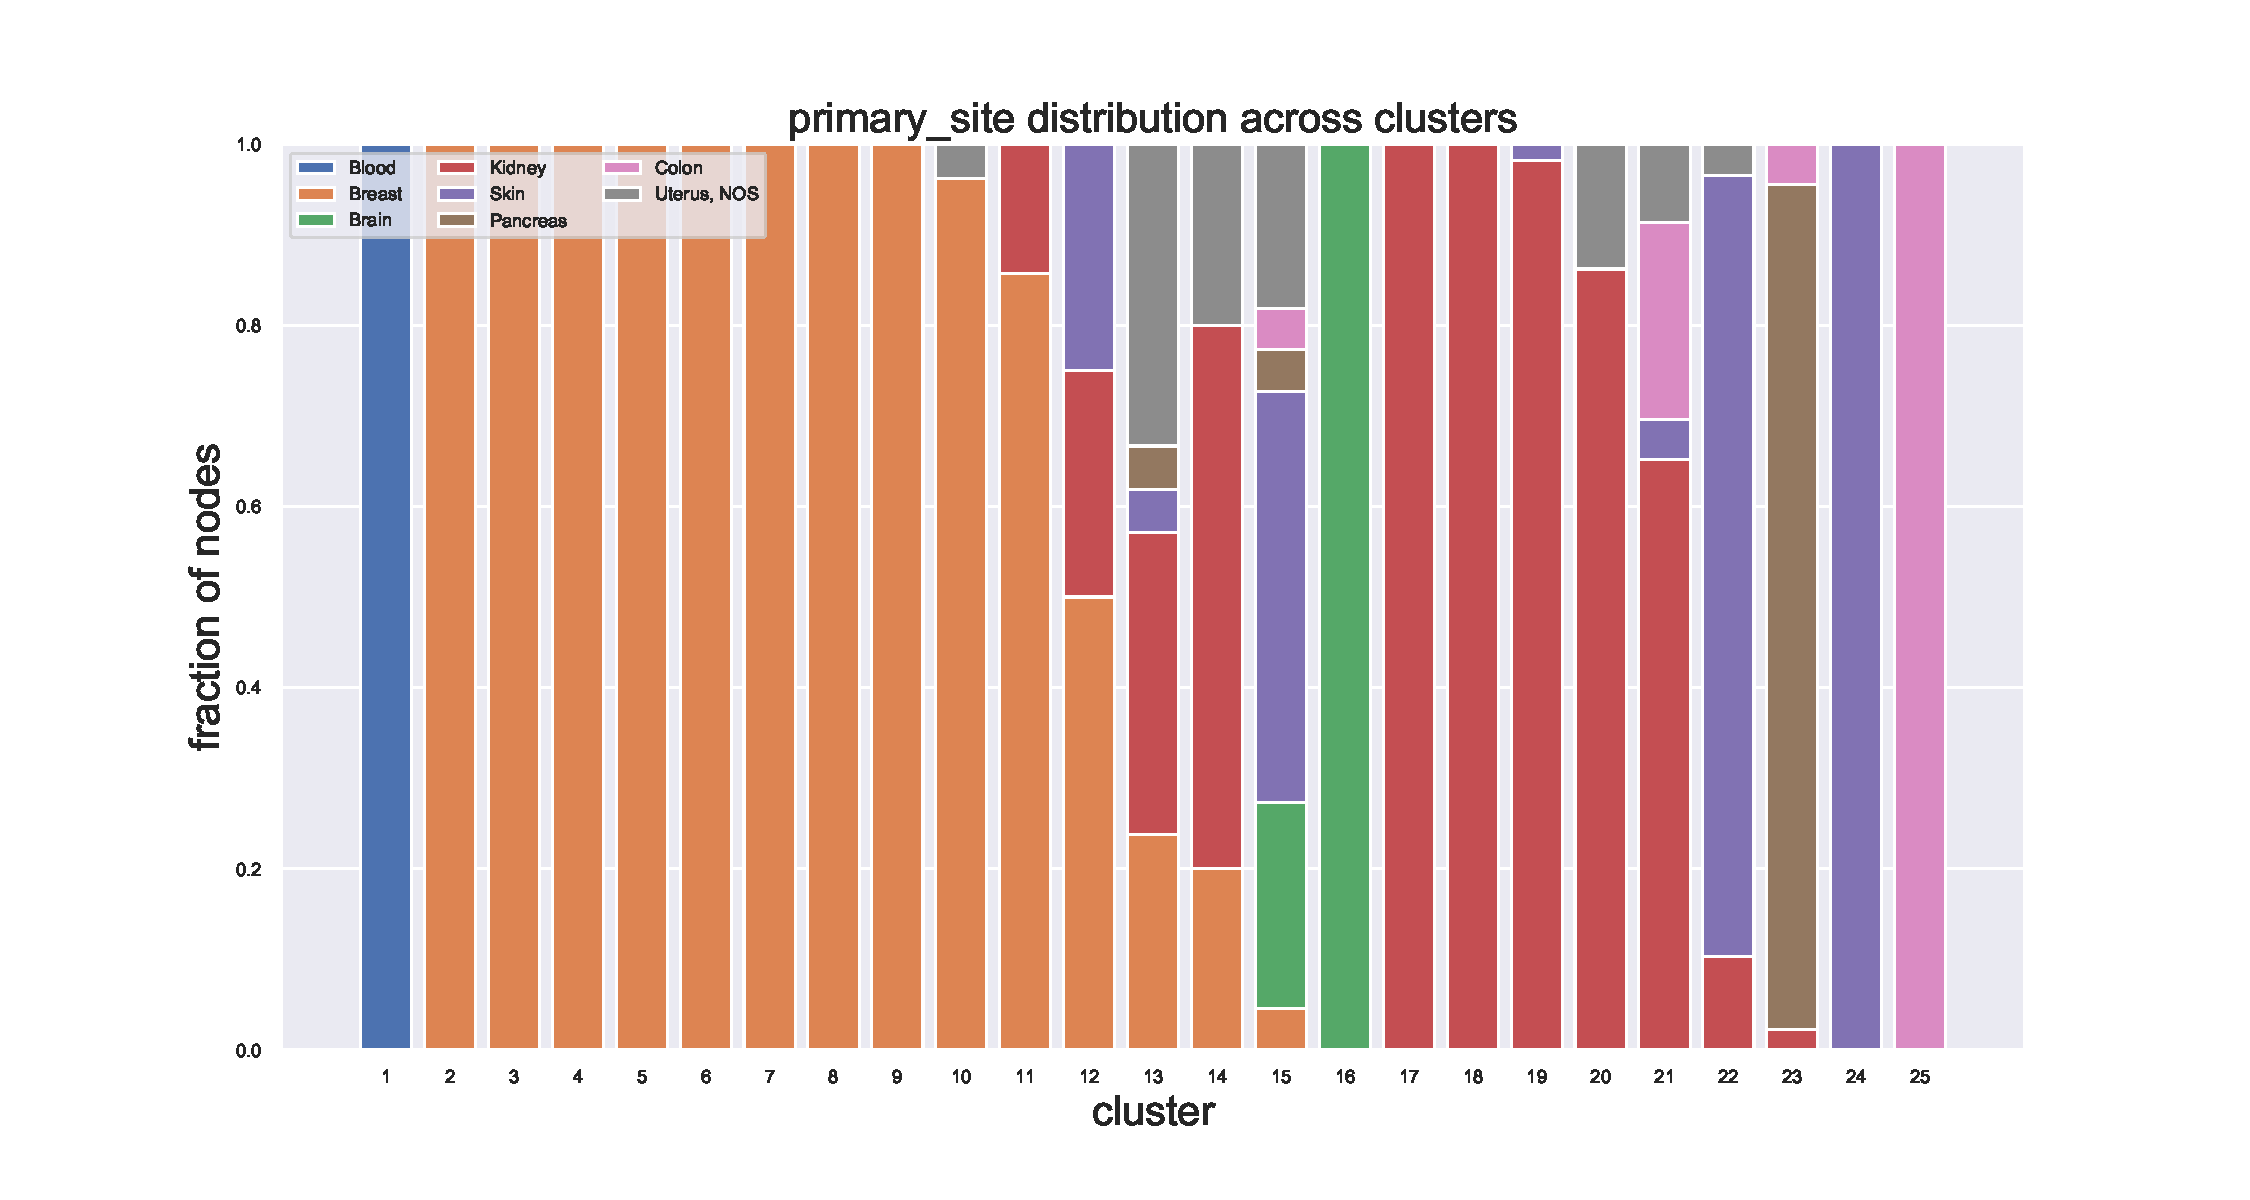
\includegraphics[width=0.9\linewidth]{pictures/topic/tcga/fraction_clustercomposition_l3_primary_site.pdf}
	\caption{Normalized cluster composition from diseased samples. The primary site is here reported.}
	\label{fig:topic/tcga/fraction_clustercomposition_l3_primary_site}
\end{figure}

Going further, deep in the hierarchy the disease type associated with each site emerges. In figure~\ref{fig:topic/tcga/fraction_clustercomposition_l2_disease_tissue} it is shown that each tissue is then separated between different disease types. Note that the pure disease type classification is not useful since certain types of tumours can happen in different sites. In this case, the power of a hierarchic approach is evident: firstly the sites are retrieved, but going further also the disease type is classified quite well.
\begin{figure}[htb!]
	\centering
	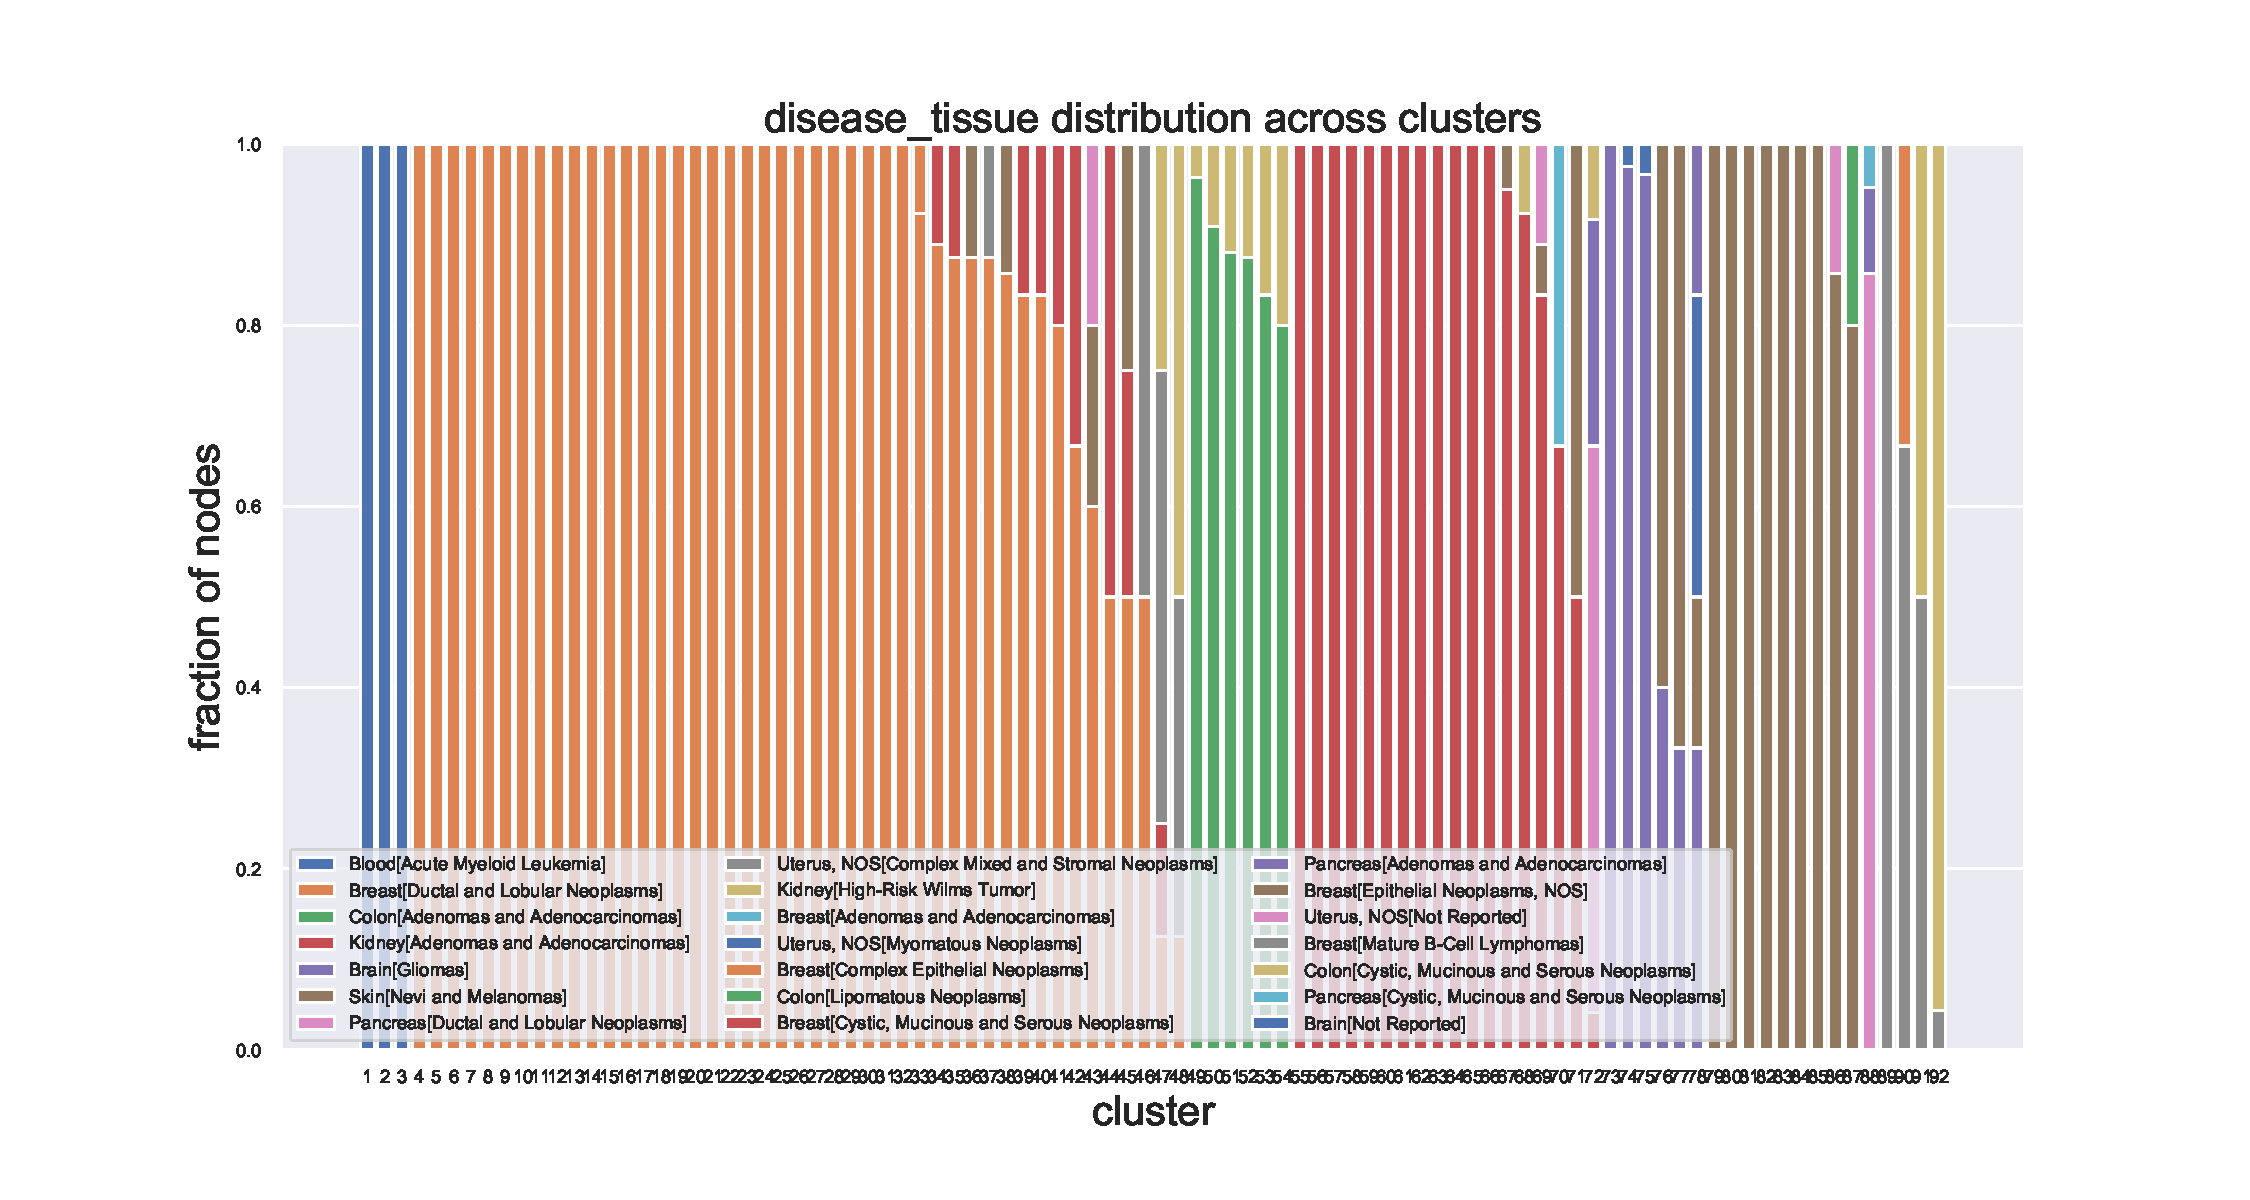
\includegraphics[width=0.9\linewidth]{pictures/topic/tcga/fraction_clustercomposition_l2_disease_tissue.pdf}
	\caption{Normalized cluster composition of diseased tissue or couple site and disease type.}
	\label{fig:topic/tcga/fraction_clustercomposition_l2_disease_tissue}
\end{figure}
\FloatBarrier
At this point when the model is demonstrated to work on healthy and diseased samples, it can be interesting to study merged healthy and diseased labels and examine how the model behaves when healthy and cancer samples are merged. It can be very useful to determine when the model identifies a diseased sample and when it is able to classify it properly.